% !TEX TS-program = pdflatex
% !TEX encoding = UTF-8 Unicode

% This is a simple template for a LaTeX document using the "article" class.
% See "book", "report", "letter" for other types of document.

\documentclass[12pt]{scrreprt} % use larger type; default would be 10pt
\linespread {1,25}\selectfont %1.25 da er von Haus aus 1.2 ist und 1,25 * 1,2 = 1,5 isch
\usepackage[utf8]{inputenc} % set input encoding (not needed with XeLaTeX)
%
%\setkomafont{chapter}{\Large\linespread{ 1}\sffamily\bfseries}
%\setkomafont{section}{\Large\linespread{ 1}\sffamily\bfseries}
%%% Examples of Article customizations
% These packages are optional, depending whether you want the features they provide.
% See the LaTeX Companion or other references for full information.

%%% PAGE DIMENSIONS
\usepackage{geometry} % to change the page dimensions
\geometry{a4paper} % or letterpaper (US) or a5paper or....
% \geometry{margin=2in} % for example, change the margins to 2 inches all round
% \geometry{landscape} % set up the page for landscape
%   read geometry.pdf for detailed page layout information

\usepackage{graphicx} % support the \includegraphics command and options

% \usepackage[parfill]{parskip} % Activate to begin paragraphs with an empty line rather than an indent

%%% PACKAGES
\usepackage[german]{babel}
\usepackage{helvet}
\usepackage{amsmath}
\usepackage{amssymb}
\usepackage{gensymb}
\usepackage{picinpar}
\usepackage{float}
\usepackage{epsfig}
\usepackage{graphicx}
\usepackage[german]{varioref}
\usepackage{natbib}
\usepackage{url}
%\usepackage{cite}
%\usepackage[round]{natbib}
%\bibliographystyle{alphadin}
%\usepackage[style=authoryear]{biblatex} %e
%\bibliographystyle{unsrt}
%\bibliography{literatur}
\usepackage{longtable} %for tables langer than a page
\usepackage{booktabs} % for much better looking tables
\usepackage{array} % for better arrays (eg matrices) in maths
\usepackage{paralist} % very flexible & customisable lists (eg. enumerate/itemize, etc.)
\usepackage{verbatim} % adds environment for commenting out blocks of text & for better verbatim
\usepackage{subfig} % make it possible to include more than one captioned figure/table in a single float
% These packages are all incorporated in the memoir class to one degree or another...

%%% HEADERS & FOOTERS
\usepackage{fancyhdr} % This should be set AFTER setting up the page geometry //fancyhdr
\pagestyle{fancy} % options: empty , plain , fancy
%\fancyhf{}
\renewcommand{\headrulewidth}{0.5pt} % customise the layout...
%\lhead{}\chead{}\rhead{}
%\lfoot{}\cfoot{\thepage}\rfoot{}
%\lohead{\headmark}


%%%% SECTION TITLE APPEARANCE
%\usepackage{sectsty}
%\allsectionsfont{\sffamily\mdseries\upshape} % (See the fntguide.pdf for font help)
% (This matches ConTeXt defaults)


\setkomafont{chapter}{\rm\bf \large} %Größe der Kapitelüberschriften
\setkomafont{section}{\rm\bf\large} %Größe der UNterkapitelüberschriften 
\setkomafont{subsection}{\rm\bf\large} %Größe der UNterkapitelüberschriften 

%%% ToC (table of contents) APPEARANCE
\usepackage[nottoc,notlof,notlot]{tocbibind} % Put the bibliography in the ToC
\usepackage[titles,subfigure]{tocloft} % Alter the style of the Table of Contents
\renewcommand{\cftsecfont}{\rmfamily\mdseries\upshape}
\renewcommand{\cftsecpagefont}{\rmfamily\mdseries\upshape} % No bold!


%\usepackage[automark]{scrpage2}
%\pagestyle{scrheadings}


%%% END Article customizations



%%% The "real" document content comes below...

\title{Entwicklung und Erprobung einer piezoresistiven Sensor-Schaltung mit drahtloser Energieversorgung im Projekt "MedLast"}
\author{Stephan Jobstmann}
\date {31. August 2012}
\pagenumbering{roman}

%\date{} % Activate to display a given date or no date (if empty),
         % otherwise the current date is printed 




\begin{document}
\maketitle
\setcounter {page}{1}
\tableofcontents
\listoffigures

\def\chapterpagestyle{fancy}

\chapter{Einleitung}
\pagenumbering{arabic}
Die moderne Schulmedizin ist mittlerweile an einem Punkt angelangt, an dem die biochemischen Prozesse innerhalb des Körpers als nahezu komplett erfasst gelten. Die Mechanismen der Informationsweitergabe über die Nervenbahnen, die Belastbarkeit der Anatomie oder die Zerlegungsprozesse des Stoffwechsels sind als solche weitestgehend erforscht. Wie jedoch in jedem Forschungsbereich bedeutet dies auch, dass die Lernkurve beziehungsweise die Anzahl der Ergebnisse an innovativen Erkenntnissen drastisch über die letzten Jahrzehnte abnehmen. Weiter lässt sich feststellen, dass die Fortschritte der modernen Medizin sich hauptsächlich auf die Innovationen aus den Bereichen der Pharmazie und der Medizintechnik berufen. So ermöglichen intelligente Kamerasysteme eine bessere Überwachung von Operationen am schlagenden Herzen oder die Abnahme von elektrischen Nervensignalen eine Steuerung von kybernetischen Prothesen.\\
Die fortschreitende Entwicklung in der Medizintechnik bietet auch Hilfestellung im Genesungsprozess im Fachbereich der Orthopädie. So wird im Projekt MedLast sowohl eine Unterstützung für den Patienten als auch eine Kontrollmöglichkeit während der Heilung einer Beinfraktur erstrebt. Dabei wird das Gewicht auf dem geschienten Fuß und die Häufigkeit der Auftritte aufgezeichnet. Gleichzeitig sollen diese Daten zur zeitnahen Kontrolle an eine visuelle Ausgabeeinheit, ähnlich einer Armbanduhr, weitergegeben werden. Da dies im Ganzen ein sehr umfangreiches Unterfangen darstellt, wird es sinngemäß in Teilbereiche untergliedert. Für die Konstruktion der Elektronik, welche die Werte für Belastung und Schrittzahl aufnimmt, werden die Gebiete Energieversorgung und Sensorik zusammengefasst. Hierbei kann man leider nur sehr schlecht auf proprietäre Komplettlösungen zurückgreifen. Darum sollen in dieser Arbeit die nötigen Schritte unternommen werden, um ein solches System zu erstellen und in Betrieb zu nehmen.
\chapter{Anforderungen}
Als wesentliche Bestandteile der Aufgabenstellung sind zuerst die zu bearbeitenden Teilgebiete zu nennen. Hierzu gehören:
\begin{itemize}
\item
Energiezuführung
\item
Energiebereitstellung
\item
Sensorik-Auswertung
\end{itemize}
Bei der Energiezuführung sollen dahingehend Überlegungen angestrebt werden, auf welche Art und Weise das komplette Modul mit Spannung versorgt werden kann. Dabei sollen autarke wie auch fremd-gespeiste Quellen betrachtet werden. Die Energiebereitstellung bezieht sich auf die Speicherung im oder am Modul selbst. Hierbei ist die Abstimmung zwischen Bedarf und Bereitstellung ausschlaggebend für die Wahl der zu verwendenden Technologie. In der Sensorik-Auswertung ist natürlich in erster Linie der zu verwendende Sensor ausschlaggebend. Da dieser sich durch den steten Optimierungsverlauf auch im Verhalten sowie in den zu erwartenden Messgrößen ändern kann, sollte diesbezüglich ein Freiheitsgrad in der Implementierung vorhanden sein. Weiter soll im zentralen Mikrocontroller des Moduls eine passende Auslesesoftware erstellt werden. Diese muss die gemessenen Daten aufbereiten und in eine passende SI-Einheit wie Newton [N] oder Kilogramm [kg] zurück rechnen. 
\chapter{Grundlagen}
\section{Energy-Harvesting}
\subsection{Piezoelektrisch}

Eines der größten abgedeckten Felder im Energy-Harvesting Bereich ist die Gewinnung von nutzbarer elektrischer Energie aus vorhandener mechanischer Energie. Hierbei werden die piezoelektrischen Effekte genutzt, welche bei Druck oder Schwingungsbelastungen auf einem Piezokristall entstehen \citep[vgl. S.36 ff]{Dembowski2011}. Dabei entsteht bei bestimmten nichtleitenden Keramiken aufgrund von mechanischem Druck elektrische Ladung an den Oberflächen. Die inneren Ladungskerne driften dabei auseinander, es bildet sich ein Dipol aus. Es werden die grundlegenden Gleichungen des Piezo-Effekts wie folgt beschrieben:
\begin{align}
D & =  \textrm{d} \cdot T + \varepsilon^{\textrm{T}} \cdot E\\
S & =  s^{\textrm{E}} \cdot T + \textrm{d} \cdot E
\end{align}
Mit den Parametern:
\begin{array}[t] {r c l}
D & : & \textrm{Dielektrische Verschiebung (statt Polarisation)}\\
S & : & \textrm{Relative mechanische Dehnung} \\
T & : &\textrm{Mechanische Spannung} \\
E & : & \textrm{Elektrische Feldstärke} \\
  $d$  & : & \textrm{piezoelektrische Ladungskonstante} \\
 s^{\textrm{E}}  & : & \textrm{Elastizitätskonstante, E = konstant} \\
 \varepsilon^{\textrm{T}}  & : & \textrm{Permittivität, T = konstant}\\
\end{array}\\ \newline
Zum Energy-Harvesting werden vorzüglich Biegebalken\footnote{im Englischen auch bekannt als Cantilever} verwendet. Diese können technologisch an die angeforderte Kraftaufnahme, die Schwingungsfrequenz und die Amplitude der resultierenden Spannung angepasst werden. Der Aufbau als Biegebalken liefert sein Optimum der Energieumwandlung bei seiner Resonanzfrequenz. Dabei unterscheidet man weiter zwischen Transversalschwingern\footnote{31-Schwingungsmodus} (Formel \ref{formel:3.3} und \ref{formel:3.4}) und Longitudinalschwingern\footnote{33-Schwingungsmodus}  (Formel \ref{formel:3.5} und \ref{formel:3.6}). 
\begin{align}
D_3 & =  \textrm{d}_{31} \cdot T_1 + \varepsilon_{33}^{\textrm{T}} \cdot E_3 \label{formel:3.3} \\
S_1 & =  s_{11}^{\textrm{E}} \cdot T_3 + \textrm{d}_{31} \cdot E_3 \label{formel:3.4}
\end{align}
Bei den Transversalschwingern wird quer zur mechanischen Auslenkung eine elektrische Spannung erzeugt. Wenn mechanische Schwingung bzw. Druckbelastung mit dem elektrischen Feld bzw. der dielektrischen Verschiebung gleichgerichtet ist, spricht man von Longitudinalschwingern. Transversalschwinger erzeugen eine rund zehnmal höhere Spannung als Longitudinalschwinger \citep[S.39]{Dembowski2011}.
\begin{align}
D_3 & =  \textrm{d}_{33} \cdot T_3 + \varepsilon_{33}^{\textrm{T}} \cdot E_3 \label{formel:3.5} \\
S_3 & =  s_{33}^{\textrm{E}} \cdot T_3 + \textrm{d}_{33} \cdot E_3 \label{formel:3.6}
\end{align}
\subsection{Thermoelektrisch}
Eine im Vergleich zu piezoelektrischem Energy-Harvesting hohe Energieumwandlung erzielt man mit der thermoelektrischen Transformation. Dabei wird als physikalische Grundlage der Seebeck-Effekt benutzt. Dieser beschreibt, dass bei zwei unterschiedlichen Metalllegierungen bei vorliegender Differenz der Temperaturen am Übergang der Elemente eine Spannung entsteht. Die entstandene Potentialdifferenz nennt man auch Thermospannung \citep[vgl. S.158]{Schruefer2012}. Die Inverse dieses Vorgangs wird mit dem Peltier-Effekt beschrieben. Da das Verhalten der spezifischen Elemente reziprok ist, kann man Peltierelemente auch zur Gewinnung von elektrischer Energie nutzen. \newline
Der Seebeck-Effekt beruht auf den folgenden molekularen Gegebenheiten: Naturgemäß wandern bei einem Metall, welches einem Temperaturunterschied ausgesetzt ist, die Elektronen von der heißen zur kalten Seite. Dies geschieht aufgrund der natürlichen Diffusionsbewegung innerhalb des Metalls. Bei zwei aneinanderliegenden, verlöteten oder verschweißten Legierungen gibt das Metall mit der niedrigeren Austrittsarbeit Elektronen an das andere Metall ab und wird dadurch positiv geladen. Dadurch bildet sich an der Kontaktfläche ein elektrisches Feld. Dieses kann resultierend als direkte Proportionale zur anliegenden Temperaturdifferenz der zwei Kontaktstellen mit einem Voltmeter gemessen werden. Übliche Werte hierfür sind ca. $10  \frac{\textrm{mV}}{100 \degree \textrm{K}}$.\newline \newline
Wenn man den technischen Aufbau nun so gestaltet, dass er zur Energieumwandlung und nicht zur Temperaturmessung verwendet werden soll, erweist es sich als zweckmäßig ein oder mehrere Peltierelemente im umgekehrten Betrieb zu verwenden. \citep[vgl. S.30]{Dembowski2011}
\chapter{Hardware}
Im Folgenden werden die Fortschritte in der Hardware-Entwicklung chronologisch und in Teilbereichen separiert aufgeführt.
\section{Energiezuführung}
Als zielführend erweist sich eine Vorüberlegung im Bezug auf die Möglichkeiten der elektrischen Speisung.
\subsection{Energy-Harvesting}
In diesem Teilbereich werden zwei physikalische Grundarten des Micro Energy Harvesting betrachtet. Diese sind die Umwandlung von mechanischer Schwingungsenergie und thermischer Differenz in elektrische Spannung. Bei der Vorbereitung und Einarbeitung in die entsprechende Thematik wird bei der Umformung von mechanischen Schwingungen in Elektrizität offensichtlich, dass dies eine ungünstige Form der Energiegewinnung für dieses System ist. Dies liegt unter anderem an der unmöglichen Abstimmung der durch den Auftritt erzeugten Erregung auf die Resonanzfrequenz des Schwingungsaufnehmers. Weiter benötigt ein solches Bauelement einen Freiraum um seine abklingende Bewegung harmonisch abbauen zu können. Es müssen auch die maximal auftretenden Beschleunigungen berücksichtigt werden was wiederum zu einer Versteifung des kompletten Federsystems führen würde. Das hätte als Resultat, dass durch die Erhöhung der dynamischen Bandbreite die verhältnismäßig kleineren Anregungen einen schlechteren Wirkungsgrad liefern würden. Diese Umstände schließen die piezoelektrische Wandlung leider für die Option der Energiezuführung aus. \citep[vgl. S.39]{Dembowski2011} \newline 
Die thermoelektrische Wandlung beruht auf der Inversen des Peltier-Effekts, dem Seebeck Effekt. Diesem liegt zu Grunde, dass am Übergang von zwei unterschiedlichen Metallen unterschiedlicher Temperierung ein elektrisches Feld aufgebaut wird. Die Verwendung dieses Effekts war zunächst nur bei Temperatur-Messfühlern weit verbreitet. Allerdings ist aufgrund der fortschreitenden Entwicklung der Micro Energy Harvesting Technologien dieser Effekt mittlerweile auch zur Energieversorgung nutzbar. \newline \newline
Als zentralen Baustein für die Erprobung von Micro-Energy-Harvesting Systemen im Bezug auf thermo-elektrische Energiewandlung bietet sich der \textbf{LTC3108} von der Firma Linear Technology an. Dieser vermag mit geringem Aufwand Eingangsspannungen von 20mV bis 500mV auf ausgangsseitig bis zu 5V aufwärts zu wandeln. Um möglichst schnell Erkenntnisse aus der Wirkungsweise des Bausteins ziehen zu können, wird eine im Internet veröffentlichte Schaltung\footnote{\url{https://github.com/wa7iut}} für Tests verwendet (siehe Abbildung \vref{fig:4.1}). Diese hält sich strikt an die Vorgaben des Datenblatts\footnote{\url{http://www.linear.com/product/LTC3108}} \citep{LTC3108}. Beim LTC3108 handelt es sich um einen Spannungs-Aufwärtswandler\footnote{Step-Up-Converter} für sehr niedrige Eingangsspannungen. Im Gegensatz zum normalen Aufbau von Aufwärtswandlern wird keine einfache Induktivität sondern ein kleiner Transformator verwendet. Dies reduziert zwar aufgrund des hohen Übersetzungsverhältnisses (1:20 bis 1:100) den Wirkungsgrad, allerdings lassen sich so auch höhere Spannungen erzeugen. Bei dem Versuchsaufbau wird ein 1:100 Transformator verwendet, da sich die Eingangsspannungen, welche experimentell ermittelt wurden, sich zwischen 20mV und 90mV bewegen. Als zu erstrebende Ausgangsspannung wurde schaltungstechnisch 3,3V eingestellt, da dies die zur Zeit am häufigsten bei Mikrocontrollern vorkommende Versorgungsspannung ist. Als externer Energiespeicher wurde ausgangsseitig an die Schaltung ein $2200 \mu$F Kondensator angefügt. Als energieerzeugendes Element wurde ein Peltierelement mit einem Aluminium-Kühlkörper versehen. So muss bei ausreichender zugeführter Wärme nicht einmal aktiv gekühlt werden, es genügt die Wärmeveräußerung durch den Kühlkörper.%weitere Fotos
\begin{figure}[htb]
\centering
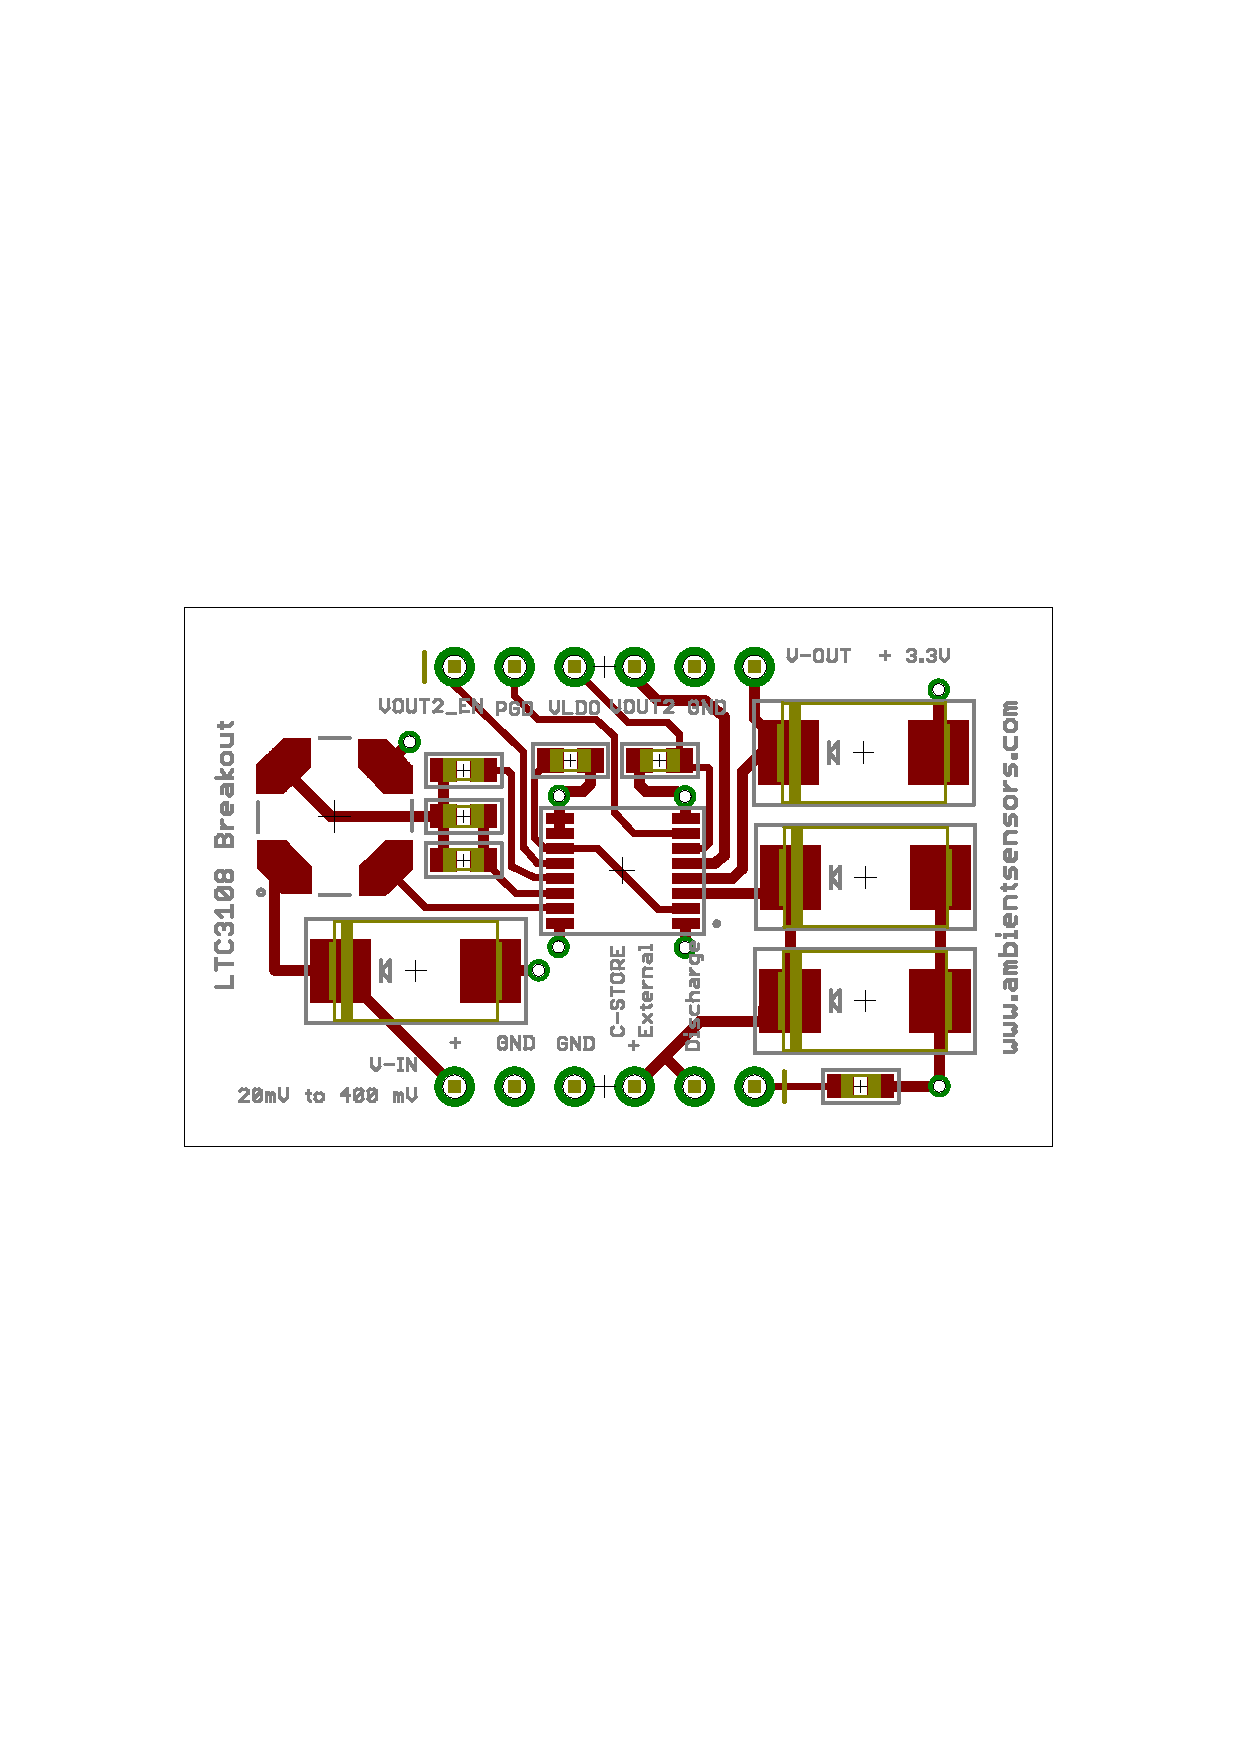
\includegraphics[bb=3.4cm 10.6cm 17.5cm 19.4cm]{Bilder/LTC3108breakoutSSOC}
\caption{LTC3108 Board von Ambient Sensors}
\label{fig:4.1}
\end{figure}
\section{Energiebereitstellung}
Da die Markttauglichkeit bei diesem Projekt eine wesentliche Rolle spielt, wird eine weitverbreitete, einfach zu realisierende und auch günstige Methode gesucht um die Energie für die Elektronik des eingebetteten Moduls bereitzustellen.
\subsection{Superkondensator}
Als Superkondensator bezeichnet man im Allgemeinen hochkapazitive Energieträger, die Ihre elektrische Ladung anders als Keramik-, Tantal-, Elektrolyt- oder Folienkondensatoren speichern. Sie funktionieren nicht wie diese durch Ladungsseparation mittels Dielektrikum sondern bedienen sich anderer Effekte, wie Energiespeicherung in Helmholtz-Doppelschichten\footnote{Doppelschichtkondensator}, faradayscher Ladungstausch\footnote{Pseudokondensator} oder einer Kombination aus beiden Technologien\footnote{Hybridkondensator}. Aufgrund dieser anderen Bauweisen lassen sich Kapazitäten erreichen, die das von Elektrolytkondensatoren um das 10000-fache überschreiten. Somit ziehen sie bezüglich der Ladungsdichte mit Akkumulatoren gleich. Anders als bei den üblichen Kondensatoren wird durch den technologischen Unterschied der Funktionsprinzipien eine lineare Lade- beziehungsweise Entladekurve erreicht. Weiter In Miniaturbauweise für Platinenmontage sind so ganzzahlige Farad an Ladungskapazität mit dieser Technologie bereits üblich. Für den praktischen Einsatz für die Arbeit fielen diese Energiespeicher aufgrund ihrer schaltungstechnischen Zusatzbeschaltung zur Spannungsstabilisierung und des, im Gegensatz zu den weit verbreiteten Lithium-Ionen Akkus, hohen Kostenfaktors aus. Weiter ist die Selbstentladung zudem höher als bei konventionellen Akkumulatoren. Aus diesen Gründen wurde eine Lösung der Energiezwischenspeicherung, welche auf Superkondensatoren basiert, nicht weiter verfolgt.
\subsection{Lithium-Ionen-Akkumulator}
 Der Lithium-Ionen-Akku hat sich in den letzten Jahren zur Standardtechnologie für wiederaufladbare Energiespeicher entwickelt. Man findet sie in nahezu jedem portablen, elektrisch betriebenen Gerät. Durch weitere Sicherheitsmaßnahmen, wie den in nahezu allen Li-Ion-Akkus verbauten NTC\footnote{Negative Temperature Coefficient}-Widerstand, der mithilfe externer Sicherheits- und Messbeschaltung Rückschlüsse über die interne Temperaturentwicklung des Energiespeichers schließen lässt. Dies verhindert bei einer Fehlfunktion oder einem Schaden des Akkus einen Brand oder gar eine Explosion des Geräts\footnote{\url{http://computer.t-online.de/} \\ \url{uelzen-explodiertes-notebook-loest-feuerwehreinsatz-aus/id_42553726/index}}. \\
Für das Projekt wurde nach einem IC-Baustein gesucht, der selbstständig bei ausreichender Eingangsspannung den Ladungsvorgang bei einem 1-Zellen Li-Ionen Akku vornimmt. Die Wahl eines fertigen ICs bietet einige Vorteile:
\begin{itemize}
\item
Der Aufbau der Schaltung reduziert sich auf ein Minimum an Bauteilen, so werden zum Beispiel Schmitt-Trigger für die Temperaturüberwachung, Spannungsstabilisatoren und Stromquellen bereits in einem Baustein vereint. 
\item
Die Komplexität des Schaltungslayouts wird auf geringen Ausmaßen festgehalten.
\item
Berechnungen zur Auslegung der einzelnen Baugruppen werden obsolet oder auf wenige reduziert. Dabei wird meistens der Anwender durch die im Datenblatt aufgezeigten Anwendungsbeispiele mit Vorlagen zur Berechnung unterstützt.
\item
Die Schaltung ist bereits im Datenblatt festgehalten und muss lediglich bei den Bauteilwerten adaptiert werden.
\end{itemize}
Nach hinreichendem Vergleich fiel die Wahl des zu verwendenden Bausteins auf den BQ24100 von der Firma Texas Instruments\footnote{\url{https://www.ti.com/product/bq24100}}. Dieser umfasst eine durch die am Akku anliegende Temperatur gesteuerte Schutzbeschaltung und eine äußerst niedrige Mindestspannung für die Eingangsbeschaltung. Weiter sind diverse Steuereingänge als auch Ausgänge die durch ihre logischen Pegel den aktuellen Status des Ladezyklus wiedergeben im Baustein realisiert. Die Ladelogik erkennt ebenfalls eine Tiefentladung und passt dementsprechend den Ladezyklus an. \\
\\
berechnung
\\
\\
Ein passendes Schaltungslayout wurde mithilfe des Datenblatts \citep{BQ24100} und der Software Multisim\footnote{\url{http://www.ni.com/multisim/d/}} erstellt. Nach der Adaption der Schaltung auf ein passendes Layout wurde über einen Leiterplattenhersteller ein Prototyp auf FR4\footnote{Flame Retarding Number 4; Flammhemmendes Substratmaterial auf Epoxydbasis} bestellt. An der Hochschule Landshut wurde dieser per Hand bestückt und mithilfe der Dampfphasenlötanlage fertig gelötet. Für erste Tests wurde ein handelsüblicher Mobiltelefon-Akku der Firma Huawei verwendet. Dieser war bereits geringfügig vorgeladen und besitzt einen internen NTC-Widerstand von 10k$\Omega$. Somit entsprach diese Testumgebung ziemlich dem realen Einsatzgebiet der Ladeschaltung. Über einen fliegenden Aufbau mithilfe einer Experimentierplatine wurde der Akku an die Schaltung angeschlossen. Diese wurde selbst an eine 5V Konstantspannungsquelle angeschlossen, welche während des Versuchs auch im Spannungspegel verändert wurde. Solange sich die anliegende Gleichspannung innerhalb des im Datenblatt vermerkten Intervalls bewegt, zeigen die Indikationsausgänge des ICs einwandfreien Betrieb auf. Die Funktion des Moduls konnte einwandfrei nachgewiesen werden und stets reproduzierbar. 
\section{Arbeitsschaltung}
\subsection{Sensorik}
Zentrales Element der Schaltung des Fußmoduls des Projekts "`MedLast"' ist der Druckaufnehmer. Erste Versuche die Druckbelastung über die Kapazitätsänderung von Piezoelementen erwiesen sich als äußerst schwierig. Die Problematik bei dieser Messmethode besteht darin, dass sie aufgrund der Flüchtigkeit der geringen Ladung und der Empfindlichkeit gegenüber parasitären Effekten äußerst aufwendig betrieben werden muss, um repräsentative und reproduzierbare Ergebnisse zu erzielen. Als parasitäre Effekte spielen hier unter anderem Luftfeuchte, Beleuchtung und die Umgebungstemperatur eine entscheidende Rolle. Bei ausführlichen Belastungstests im Bereich bis 200N konnten keine zufriedenstellenden Ergebnisse erzielt werden \citep{Jobstmann2012}. \newline
Darum wurde die Messmethode auf piezoresistive Dehnungsmessstreifen geändert. Diese Technologie bietet auch den Vorteil, dass aufgrund der eigenen Labor Verarbeitung im Hybridlabor der Hochschule Landshut das Layout beliebig angepasst werden. 
\bibliography{literatur}
\bibliographystyle{alpha}
\end{document}